
%% bare_jrnl_transmag.tex
%% V1.4b
%% 2015/08/26
%% by Michael Shell
%% see http://www.michaelshell.org/
%% for current contact information.
%%
%% This is a skeleton file demonstrating the use of IEEEtran.cls
%% (requires IEEEtran.cls version 1.8b or later) with an IEEE 
%% Transactions on Magnetics journal paper.
%%
%% Support sites:
%% http://www.michaelshell.org/tex/ieeetran/
%% http://www.ctan.org/pkg/ieeetran
%% and
%% http://www.ieee.org/

%%*************************************************************************
%% Legal Notice:
%% This code is offered as-is without any warranty either expressed or
%% implied; without even the implied warranty of MERCHANTABILITY or
%% FITNESS FOR A PARTICULAR PURPOSE! 
%% User assumes all risk.
%% In no event shall the IEEE or any contributor to this code be liable for
%% any damages or losses, including, but not limited to, incidental,
%% consequential, or any other damages, resulting from the use or misuse
%% of any information contained here.
%%
%% All comments are the opinions of their respective authors and are not
%% necessarily endorsed by the IEEE.
%%
%% This work is distributed under the LaTeX Project Public License (LPPL)
%% ( http://www.latex-project.org/ ) version 1.3, and may be freely used,
%% distributed and modified. A copy of the LPPL, version 1.3, is included
%% in the base LaTeX documentation of all distributions of LaTeX released
%% 2003/12/01 or later.
%% Retain all contribution notices and credits.
%% ** Modified files should be clearly indicated as such, including  **
%% ** renaming them and changing author support contact information. **
%%*************************************************************************


% *** Authors should verify (and, if needed, correct) their LaTeX system  ***
% *** with the testflow diagnostic prior to trusting their LaTeX platform ***
% *** with production work. The IEEE's font choices and paper sizes can   ***
% *** trigger bugs that do not appear when using other class files.       ***                          ***
% The testflow support page is at:
% http://www.michaelshell.org/tex/testflow/



\documentclass[journal,transmag]{IEEEtran}
%\usepackage[style=authoryear,backend=bibtex]{biblatex} %backend tells biblatex what you will be using to process the bibliography file
%\addbibresource{refer.bib}
\usepackage{graphicx}
%
% If IEEEtran.cls has not been installed into the LaTeX system files,
% manually specify the path to it like:
% \documentclass[journal]{../sty/IEEEtran}





% Some very useful LaTeX packages include:
% (uncomment the ones you want to load)


% *** MISC UTILITY PACKAGES ***
%
%\usepackage{ifpdf}
% Heiko Oberdiek's ifpdf.sty is very useful if you need conditional
% compilation based on whether the output is pdf or dvi.
% usage:
% \ifpdf
%   % pdf code
% \else
%   % dvi code
% \fi
% The latest version of ifpdf.sty can be obtained from:
% http://www.ctan.org/pkg/ifpdf
% Also, note that IEEEtran.cls V1.7 and later provides a builtin
% \ifCLASSINFOpdf conditional that works the same way.
% When switching from latex to pdflatex and vice-versa, the compiler may
% have to be run twice to clear warning/error messages.






% *** CITATION PACKAGES ***
%
\usepackage{cite}
% cite.sty was written by Donald Arseneau
% V1.6 and later of IEEEtran pre-defines the format of the cite.sty package
% \cite{} output to follow that of the IEEE. Loading the cite package will
% result in citation numbers being automatically sorted and properly
% "compressed/ranged". e.g., [1], [9], [2], [7], [5], [6] without using
% cite.sty will become [1], [2], [5]--[7], [9] using cite.sty. cite.sty's
% \cite will automatically add leading space, if needed. Use cite.sty's
% noadjust option (cite.sty V3.8 and later) if you want to turn this off
% such as if a citation ever needs to be enclosed in parenthesis.
% cite.sty is already installed on most LaTeX systems. Be sure and use
% version 5.0 (2009-03-20) and later if using hyperref.sty.
% The latest version can be obtained at:
% http://www.ctan.org/pkg/cite
% The documentation is contained in the cite.sty file itself.






% *** GRAPHICS RELATED PACKAGES ***
%
\ifCLASSINFOpdf
  % \usepackage[pdftex]{graphicx}
  % declare the path(s) where your graphic files are
  % \graphicspath{{../pdf/}{../jpeg/}}
  % and their extensions so you won't have to specify these with
  % every instance of \includegraphics
  % \DeclareGraphicsExtensions{.pdf,.jpeg,.png}
\else
  % or other class option (dvipsone, dvipdf, if not using dvips). graphicx
  % will default to the driver specified in the system graphics.cfg if no
  % driver is specified.
  % \usepackage[dvips]{graphicx}
  % declare the path(s) where your graphic files are
  % \graphicspath{{../eps/}}
  % and their extensions so you won't have to specify these with
  % every instance of \includegraphics
  % \DeclareGraphicsExtensions{.eps}
\fi
% graphicx was written by David Carlisle and Sebastian Rahtz. It is
% required if you want graphics, photos, etc. graphicx.sty is already
% installed on most LaTeX systems. The latest version and documentation
% can be obtained at: 
% http://www.ctan.org/pkg/graphicx
% Another good source of documentation is "Using Imported Graphics in
% LaTeX2e" by Keith Reckdahl which can be found at:
% http://www.ctan.org/pkg/epslatex
%
% latex, and pdflatex in dvi mode, support graphics in encapsulated
% postscript (.eps) format. pdflatex in pdf mode supports graphics
% in .pdf, .jpeg, .png and .mps (metapost) formats. Users should ensure
% that all non-photo figures use a vector format (.eps, .pdf, .mps) and
% not a bitmapped formats (.jpeg, .png). The IEEE frowns on bitmapped formats
% which can result in "jaggedy"/blurry rendering of lines and letters as
% well as large increases in file sizes.
%
% You can find documentation about the pdfTeX application at:
% http://www.tug.org/applications/pdftex




% *** MATH PACKAGES ***
%
%\usepackage{amsmath}
% A popular package from the American Mathematical Society that provides
% many useful and powerful commands for dealing with mathematics.
%
% Note that the amsmath package sets \interdisplaylinepenalty to 10000
% thus preventing page breaks from occurring within multiline equations. Use:
%\interdisplaylinepenalty=2500
% after loading amsmath to restore such page breaks as IEEEtran.cls normally
% does. amsmath.sty is already installed on most LaTeX systems. The latest
% version and documentation can be obtained at:
% http://www.ctan.org/pkg/amsmath





% *** SPECIALIZED LIST PACKAGES ***
%
%\usepackage{algorithmic}
% algorithmic.sty was written by Peter Williams and Rogerio Brito.
% This package provides an algorithmic environment fo describing algorithms.
% You can use the algorithmic environment in-text or within a figure
% environment to provide for a floating algorithm. Do NOT use the algorithm
% floating environment provided by algorithm.sty (by the same authors) or
% algorithm2e.sty (by Christophe Fiorio) as the IEEE does not use dedicated
% algorithm float types and packages that provide these will not provide
% correct IEEE style captions. The latest version and documentation of
% algorithmic.sty can be obtained at:
% http://www.ctan.org/pkg/algorithms
% Also of interest may be the (relatively newer and more customizable)
% algorithmicx.sty package by Szasz Janos:
% http://www.ctan.org/pkg/algorithmicx




% *** ALIGNMENT PACKAGES ***
%
%\usepackage{array}
% Frank Mittelbach's and David Carlisle's array.sty patches and improves
% the standard LaTeX2e array and tabular environments to provide better
% appearance and additional user controls. As the default LaTeX2e table
% generation code is lacking to the point of almost being broken with
% respect to the quality of the end results, all users are strongly
% advised to use an enhanced (at the very least that provided by array.sty)
% set of table tools. array.sty is already installed on most systems. The
% latest version and documentation can be obtained at:
% http://www.ctan.org/pkg/array


% IEEEtran contains the IEEEeqnarray family of commands that can be used to
% generate multiline equations as well as matrices, tables, etc., of high
% quality.




% *** SUBFIGURE PACKAGES ***
%\ifCLASSOPTIONcompsoc
%  \usepackage[caption=false,font=normalsize,labelfont=sf,textfont=sf]{subfig}
%\else
%  \usepackage[caption=false,font=footnotesize]{subfig}
%\fi
% subfig.sty, written by Steven Douglas Cochran, is the modern replacement
% for subfigure.sty, the latter of which is no longer maintained and is
% incompatible with some LaTeX packages including fixltx2e. However,
% subfig.sty requires and automatically loads Axel Sommerfeldt's caption.sty
% which will override IEEEtran.cls' handling of captions and this will result
% in non-IEEE style figure/table captions. To prevent this problem, be sure
% and invoke subfig.sty's "caption=false" package option (available since
% subfig.sty version 1.3, 2005/06/28) as this is will preserve IEEEtran.cls
% handling of captions.
% Note that the Computer Society format requires a larger sans serif font
% than the serif footnote size font used in traditional IEEE formatting
% and thus the need to invoke different subfig.sty package options depending
% on whether compsoc mode has been enabled.
%
% The latest version and documentation of subfig.sty can be obtained at:
% http://www.ctan.org/pkg/subfig



% *** FLOAT PACKAGES ***
%
%\usepackage{fixltx2e}
% fixltx2e, the successor to the earlier fix2col.sty, was written by
% Frank Mittelbach and David Carlisle. This package corrects a few problems
% in the LaTeX2e kernel, the most notable of which is that in current
% LaTeX2e releases, the ordering of single and double column floats is not
% guaranteed to be preserved. Thus, an unpatched LaTeX2e can allow a
% single column figure to be placed prior to an earlier double column
% figure.
% Be aware that LaTeX2e kernels dated 2015 and later have fixltx2e.sty's
% corrections already built into the system in which case a warning will
% be issued if an attempt is made to load fixltx2e.sty as it is no longer
% needed.
% The latest version and documentation can be found at:
% http://www.ctan.org/pkg/fixltx2e


%\usepackage{stfloats}
% stfloats.sty was written by Sigitas Tolusis. This package gives LaTeX2e
% the ability to do double column floats at the bottom of the page as well
% as the top. (e.g., "\begin{figure*}[!b]" is not normally possible in
% LaTeX2e). It also provides a command:
%\fnbelowfloat
% to enable the placement of footnotes below bottom floats (the standard
% LaTeX2e kernel puts them above bottom floats). This is an invasive package
% which rewrites many portions of the LaTeX2e float routines. It may not work
% with other packages that modify the LaTeX2e float routines. The latest
% version and documentation can be obtained at:
% http://www.ctan.org/pkg/stfloats
% Do not use the stfloats baselinefloat ability as the IEEE does not allow
% \baselineskip to stretch. Authors submitting work to the IEEE should note
% that the IEEE rarely uses double column equations and that authors should try
% to avoid such use. Do not be tempted to use the cuted.sty or midfloat.sty
% packages (also by Sigitas Tolusis) as the IEEE does not format its papers in
% such ways.
% Do not attempt to use stfloats with fixltx2e as they are incompatible.
% Instead, use Morten Hogholm'a dblfloatfix which combines the features
% of both fixltx2e and stfloats:
%
% \usepackage{dblfloatfix}
% The latest version can be found at:
% http://www.ctan.org/pkg/dblfloatfix




%\ifCLASSOPTIONcaptionsoff
%  \usepackage[nomarkers]{endfloat}
% \let\MYoriglatexcaption\caption
% \renewcommand{\caption}[2][\relax]{\MYoriglatexcaption[#2]{#2}}
%\fi
% endfloat.sty was written by James Darrell McCauley, Jeff Goldberg and 
% Axel Sommerfeldt. This package may be useful when used in conjunction with 
% IEEEtran.cls'  captionsoff option. Some IEEE journals/societies require that
% submissions have lists of figures/tables at the end of the paper and that
% figures/tables without any captions are placed on a page by themselves at
% the end of the document. If needed, the draftcls IEEEtran class option or
% \CLASSINPUTbaselinestretch interface can be used to increase the line
% spacing as well. Be sure and use the nomarkers option of endfloat to
% prevent endfloat from "marking" where the figures would have been placed
% in the text. The two hack lines of code above are a slight modification of
% that suggested by in the endfloat docs (section 8.4.1) to ensure that
% the full captions always appear in the list of figures/tables - even if
% the user used the short optional argument of \caption[]{}.
% IEEE papers do not typically make use of \caption[]'s optional argument,
% so this should not be an issue. A similar trick can be used to disable
% captions of packages such as subfig.sty that lack options to turn off
% the subcaptions:
% For subfig.sty:
% \let\MYorigsubfloat\subfloat
% \renewcommand{\subfloat}[2][\relax]{\MYorigsubfloat[]{#2}}
% However, the above trick will not work if both optional arguments of
% the \subfloat command are used. Furthermore, there needs to be a
% description of each subfigure *somewhere* and endfloat does not add
% subfigure captions to its list of figures. Thus, the best approach is to
% avoid the use of subfigure captions (many IEEE journals avoid them anyway)
% and instead reference/explain all the subfigures within the main caption.
% The latest version of endfloat.sty and its documentation can obtained at:
% http://www.ctan.org/pkg/endfloat
%
% The IEEEtran \ifCLASSOPTIONcaptionsoff conditional can also be used
% later in the document, say, to conditionally put the References on a 
% page by themselves.




% *** PDF, URL AND HYPERLINK PACKAGES ***
%
%\usepackage{url}
% url.sty was written by Donald Arseneau. It provides better support for
% handling and breaking URLs. url.sty is already installed on most LaTeX
% systems. The latest version and documentation can be obtained at:
% http://www.ctan.org/pkg/url
% Basically, \url{my_url_here}.




% *** Do not adjust lengths that control margins, column widths, etc. ***
% *** Do not use packages that alter fonts (such as pslatex).         ***
% There should be no need to do such things with IEEEtran.cls V1.6 and later.
% (Unless specifically asked to do so by the journal or conference you plan
% to submit to, of course. )


% correct bad hyphenation here
\hyphenation{op-tical net-works semi-conduc-tor}


\begin{document}
%
% paper title
% Titles are generally capitalized except for words such as a, an, and, as,
% at, but, by, for, in, nor, of, on, or, the, to and up, which are usually
% not capitalized unless they are the first or last word of the title.
% Linebreaks \\ can be used within to get better formatting as desired.
% Do not put math or special symbols in the title.
\title{Indoor Localization system using Time of Flight in UWB spectrum}

% author names and affiliations
% transmag papers use the long conference author name format.

\author{\IEEEauthorblockN{Anirban Ghosh,
Albert Davies,
Tejus Siddagangaiah}
\IEEEauthorblockA{Electrical and Computer Engineering Department,
Carnegie Mellon University, Pittsburgh, PA 15213 USA}}




% The paper headers
%\markboth{Journal of \LaTeX\ Class Files,~Vol.~14, No.~8, August~2015}%
%{Shell \MakeLowercase{\textit{et al.}}: Bare Demo of IEEEtran.cls for IEEE Transactions on Magnetics Journals}
% The only time the second header will appear is for the odd numbered pages
% after the title page when using the twoside option.
% 
% *** Note that you probably will NOT want to include the author's ***
% *** name in the headers of peer review papers.                   ***
% You can use \ifCLASSOPTIONpeerreview for conditional compilation here if
% you desire.




% If you want to put a publisher's ID mark on the page you can do it like
% this:
%\IEEEpubid{0000--0000/00\$00.00~\copyright~2015 IEEE}
% Remember, if you use this you must call \IEEEpubidadjcol in the second
% column for its text to clear the IEEEpubid mark.



% use for special paper notices
%\IEEEspecialpapernotice{(Invited Paper)}


% for Transactions on Magnetics papers, we must declare the abstract and
% index terms PRIOR to the title within the \IEEEtitleabstractindextext
% IEEEtran command as these need to go into the title area created by
% \maketitle.
% As a general rule, do not put math, special symbols or citations
% in the abstract or keywords.
%\IEEEtitleabstractindextext{%
%\begin{abstract}
%The abstract goes here.
%\end{abstract}

% Note that keywords are not normally used for peerreview papers.
%\begin{IEEEkeywords}
%IEEE, IEEEtran, IEEE Transactions on Magnetics, journal, \LaTeX, %magnetics, paper, template.
%\end{IEEEkeywords}}



% make the title area
\maketitle


% To allow for easy dual compilation without having to reenter the
% abstract/keywords data, the \IEEEtitleabstractindextext text will
% not be used in maketitle, but will appear (i.e., to be "transported")
% here as \IEEEdisplaynontitleabstractindextext when the compsoc 
% or transmag modes are not selected <OR> if conference mode is selected 
% - because all conference papers position the abstract like regular
% papers do.
\IEEEdisplaynontitleabstractindextext
% \IEEEdisplaynontitleabstractindextext has no effect when using
% compsoc or transmag under a non-conference mode.







% For peer review papers, you can put extra information on the cover
% page as needed:
% \ifCLASSOPTIONpeerreview
% \begin{center} \bfseries EDICS Category: 3-BBND \end{center}
% \fi
%
% For peerreview papers, this IEEEtran command inserts a page break and
% creates the second title. It will be ignored for other modes.
\IEEEpeerreviewmaketitle



\section{Motivation}
Positioning systems based on GPS have become ubiquitous over the past few decades. Due to the attenuation of GPS signals by concrete walls, they cannot be used in an indoor setting for localization. In recent years, multiple attempts have been made to design a localization system for indoor applications. Indoor localization has the potential for trans-formative impact in a wide variety of applications like augmented reality, indoor navigation and advertising. Due to the inherent nature of the applications, high accuracy as well as energy efficiency is required.

Based on the application in target, various methods and system architectures have been proposed using broadcast-based technologies(RFID\cite{bouet2008rfid}, BLE\cite{alps}, WiFi\cite{yang2012locating}, Ultrasound\cite{ultrasonic}) and motion based algorithms(Inertial based sensing)\cite{li2012reliable}. The choice of the algorithm and system architecture is an integral part of solving this problem as these choices directly impact both accuracy and energy consumption of the system. 

\section{Methodology}
In our project, we propose and implement a system which is both accurate enough and energy efficient to be powered by batteries. The proposed method uses Time of Flight(TOF) algorithm to calculate the distance between two nodes. Although, TOF requires high time-synchronization and accurate time-stamping, we expect to achieve good results with this approach using the Decawave DW1000 sensors. The manufacturer claims a distance measurement accuracy within 10cm using these sensors.  The block diagram of CC3200 and DW1000 are shown in figures \ref{CC3200BD} and \ref{DW1000BD}.

\begin{figure}[!h]
\centering
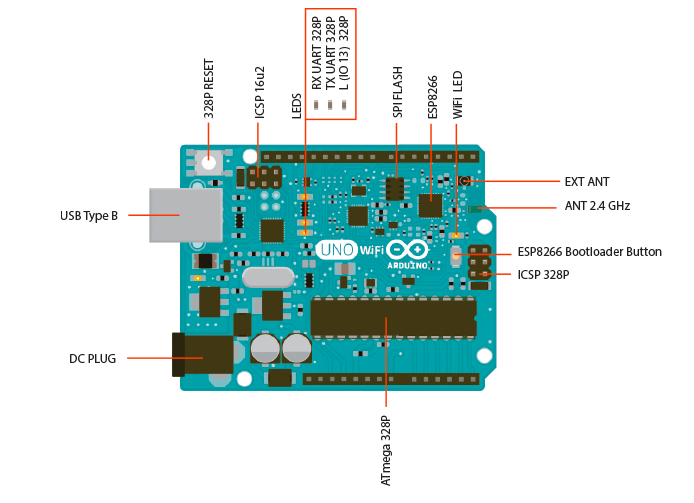
\includegraphics[width=2.5in]{arduinounobd}
\caption{{Block Diagram of CC3200 SoC}}
\label{CC3200BD}
\end{figure}


\begin{figure}[!t]
\centering
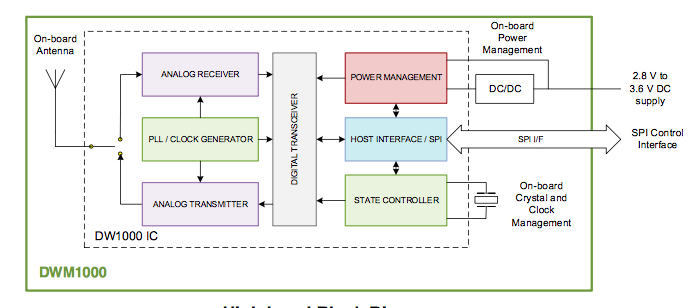
\includegraphics[width=3.5in]{dw1000bd}
\caption{{Block Diagram of DW1000 UWB transceiver}}
\label{DW1000BD}
\end{figure}

We can localize any node if we know the distance of the node from 3 or more fixed anchor points. In the TOF approach, every node that we are trying to localize, transmits packets to a set of anchored nodes whose locations are known. The anchor nodes reply with the appropriate timestamps. Using the time taken for roundtrip the distance between pairs of nodes can be calculated. Once the distance of the mobile node from each of the anchor nodes is determined, the co-ordinates of the mobile nodes can be triangulated in 3 dimensions.

To obtain the distance measurements, we having chosen to use time of flight of radio over UWB spectrum. UWB involves sending very short spikes of radio signals. This provides significant benefits like fine time resolution, energy efficiency and robustness to interference in harsh environments \cite{IEEE4}. UWB is also particularly resistant to Multi-Path effects. In this project we plan to use DecaWave ScenSor DWM1000 Modules for UWB TOF measurements. We plan to have both our mobile and anchor nodes as DWM1000 modules. Using these modules the distance of the mobile node from each of the anchor nodes can be determined.  This information has to be accumulated at a gateway for the co-ordinate computation. For this we plan to interface DWM1000 with an appropriate MCU platform using the SPI interface supported by DWM1000.

%Describe why CC3200.
\begin{figure}[!t]
\centering
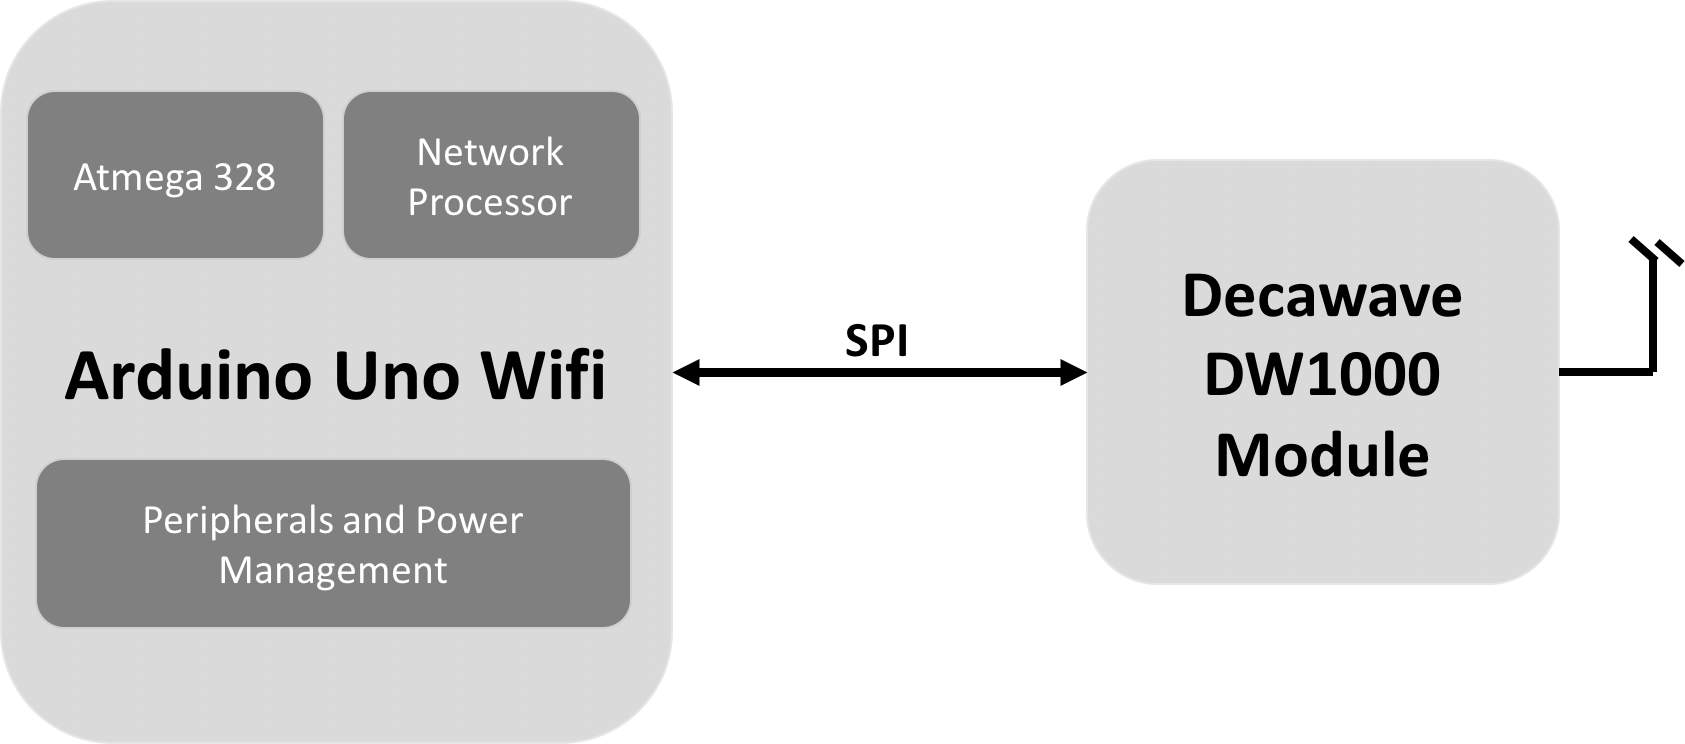
\includegraphics[width=3.5in]{nodebd.png}
\caption{{System Block Diagram of Each Node}}
\label{EACHNODEBD}
\end{figure}

A single chip Wireless MCU - CC3200 from Texas Instruments will be used to configure the sensor and run our application. The CC3200 SoC comes with a inbuilt WiFi module which can be used to interface with a PC to log the data and monitor all the nodes.

CC3200 is a WiFi Certified single chip Micro controller unit with built-in 2.4GHz PHY/MAC and TCP/IP networking engine. The controller provides a easy to use framework with wide variety of peripherals. Multiple Real-Time Operating systems like FreeRTOS and TIRTOS are supported for this platform. Although, we do not plan to use many of these features, the platform/software can be scaled to implement complex algorithms and capabilities in the future. The network engine on this controller can be configured to behave as an access point or as a host. A mobile device or a personal computer can connect to the SoC when configured as an access point. We plan to use this capability to log data and monitor all the mobile nodes. In our architecture, the mobile node transfers all the data(time stamps from each anchor node) to a personal computer(gateway). This gateway then uses these pairwise distance measurements to compute the co-ordinates of the mobile node. A software application running on the computer, logs this data and displays the location of the mobile nodes on a GUI. 

\begin{figure}[!h]
\centering
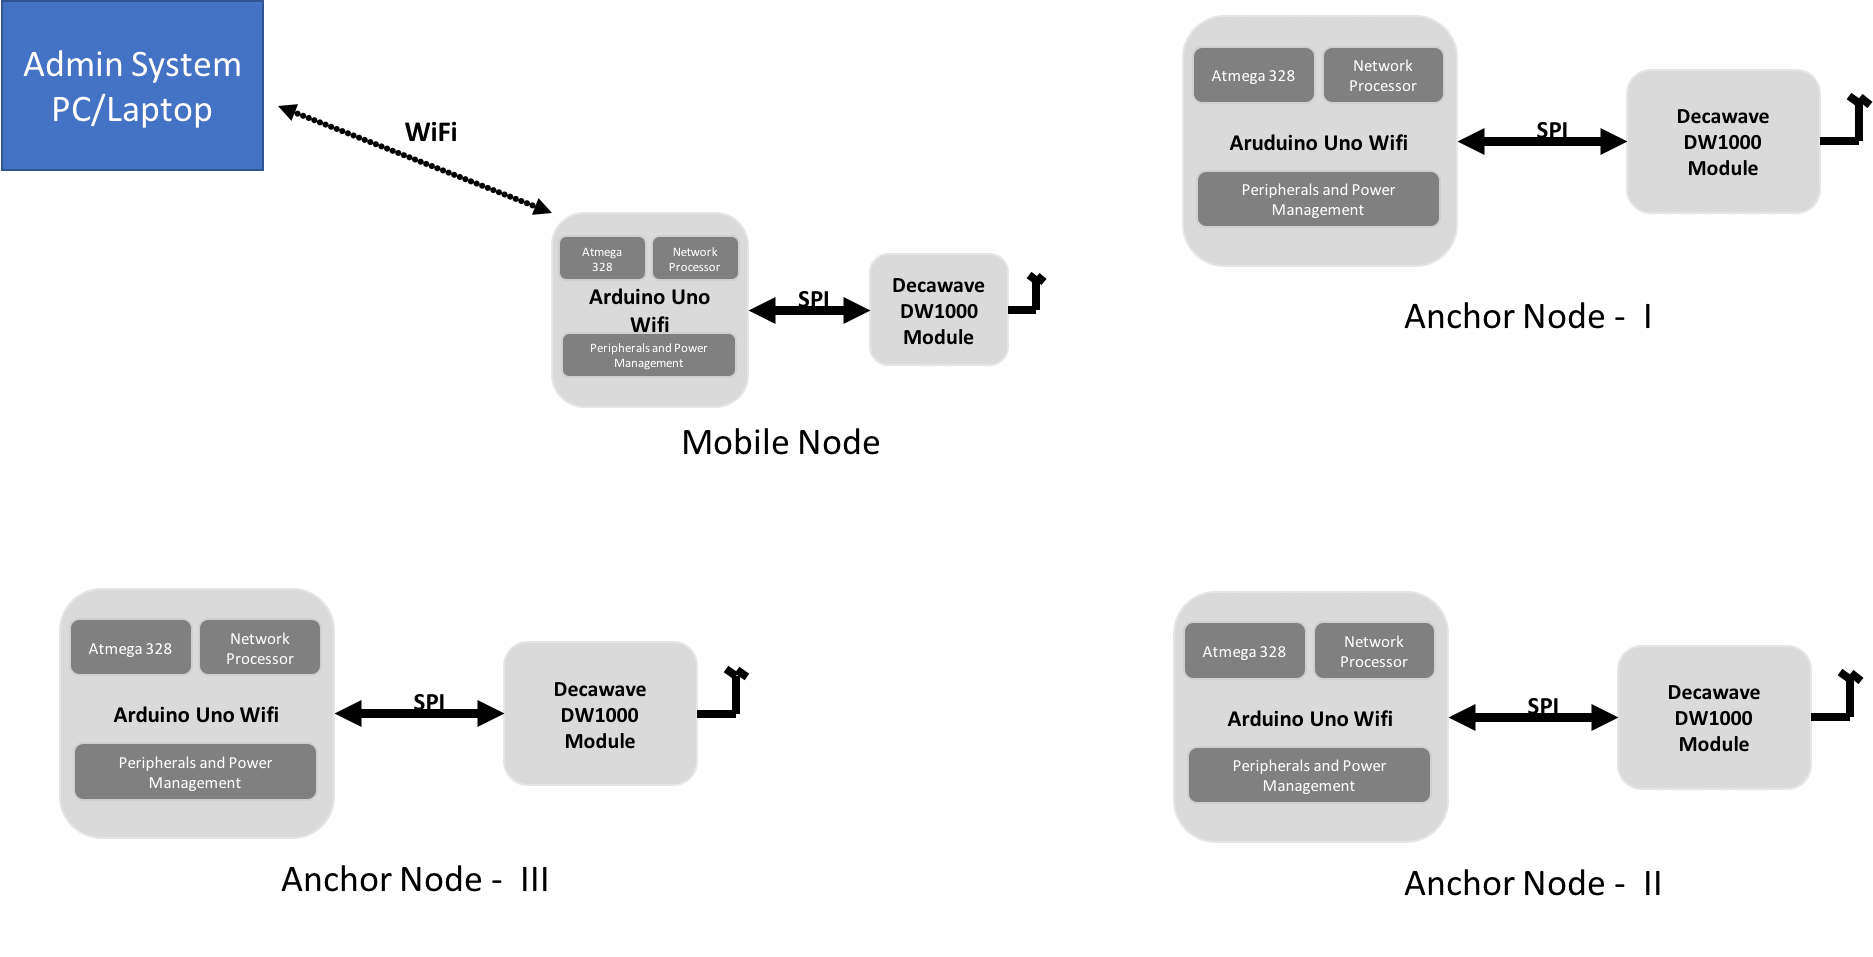
\includegraphics[width=3.5in]{sysbd.png}
\caption{{Complete system architecture}}
\label{SYSTEMBD}
\end{figure}

One disadvantage of using ToF algorithm is that it cannot be scaled. As the number of nodes increase, we expect each node to consume more energy. As an extended goal, we propose to use Time Difference of Arrival(TDOA)\cite{anthonyrowe's paper} to provide scalability. In this system architecture, anchor nodes will broadcast their location to all the nodes that are being localized in the vicinity. Using the anchor node's location and the difference in time of arrival of packets from each of the anchor nodes, triangulation can be performed. A detailed explanation of these algorithms are provided in the next section.

\section{Implementation}
As show in figure \ref{SYSTEMBD}, we use multiple anchor nodes with known positions to locate a mobile tag node. We use dynamic network discovery to connect tags with anchor nodes and perform 2-way ranging with each anchor node. The calculated distance between the tag and each anchor is sent from the tag to an admin laptop over WiFi. The distances from four anchor nodes is used to perform localization. The error of localization in our implementation is as less as 10 cm on each axis in the best case. On an average, we are able to locate the mobile node within a 20 cm error on all three axes. 
\subsection{Network Discovery and Communication}
A mobile tag node performs network discovery and initiates 2-way ranging with each of the anchor nodes. \textit{TAG} node controls the entire network to calculate the point-to-point distance betwee the anchor node and itself. As soon as the \textit{TAG} node is turned on, it broadcasts a \textbf{POLL} packet to all its neighbours. All the \textit{ANCHOR} nodes that receive the broadcast packet, respond with a \textbf{POLL\_ACK} message. The mobile node uses these acknowledgement messages to prepare a list of anchor nodes in its range. It is important to note that the mobile node sends one broadcast message and received multiple acknowledgment messages.\\  
\begin{figure}[!h]
\centering
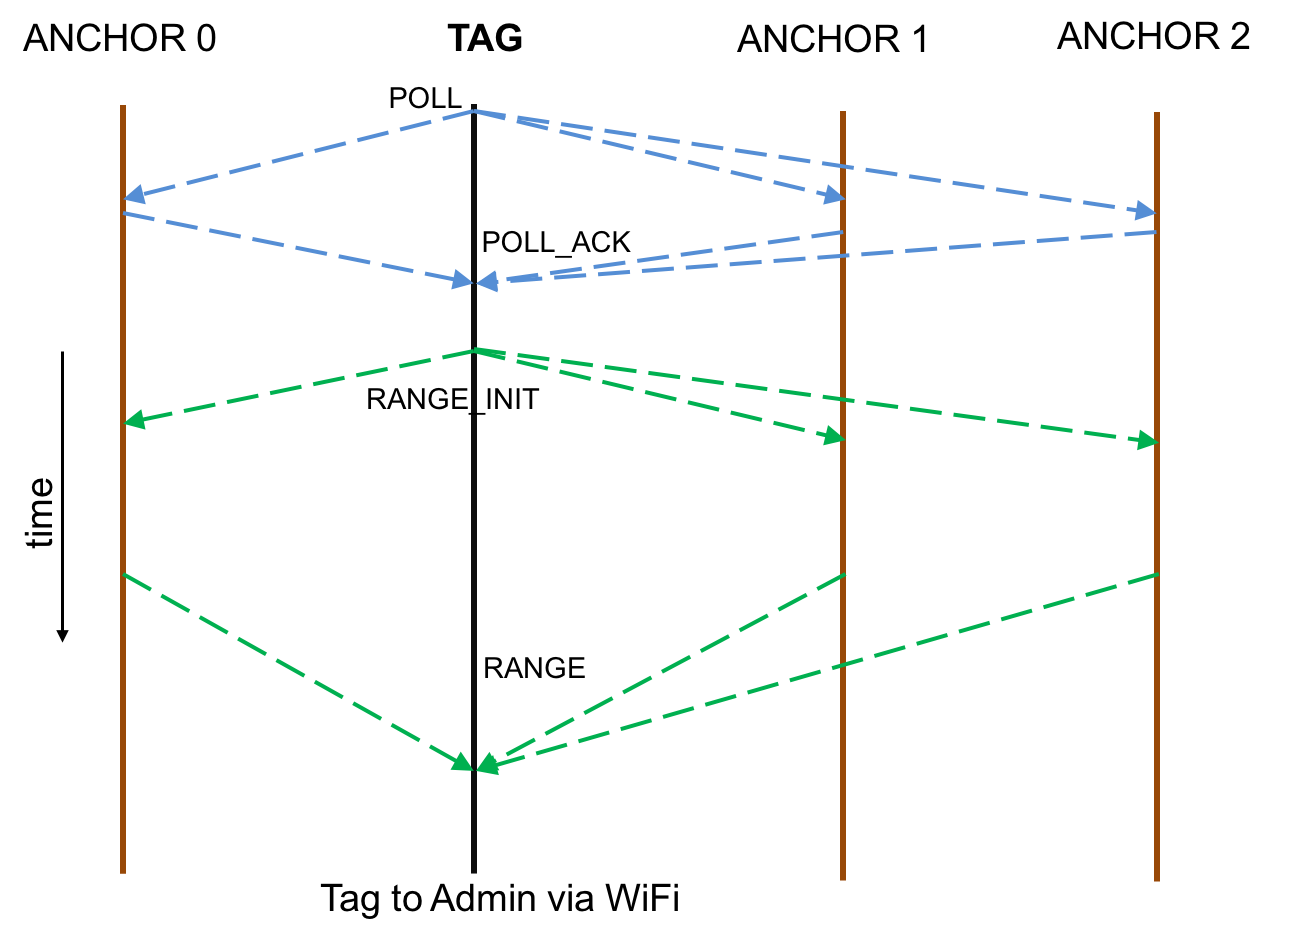
\includegraphics[width=3.5in]{communication.png}
\caption{{Network discovery and two-way ranging protocol}}
\label{commsystem}
\end{figure}
Using the network discovery performed using \textbf{POLL} and \textbf{POLL\_ACK} messages, the mobile node maintains a list of anchor nodes and performs 2-way ranging with each of those nodes. Once the anchor nodes respond with \textbf{POLL\_ACK} message, it waits to receive the \textbf{RANGE\_INIT} packet from the mobile node. \textbf{RANGE\_INIT} and \textbf{RANGE} packets are exchanged between the nodes using timestamps to perform 2-way ranging. As shown in figure \ref{commsystem} the messages exchanged between the mobile node and the anchor nodes involve multiple steps and are performed one after the other. 

If an anchor node goes out of range after responding with the acknowledgement message, the mobile node marks it as an inactive node and deletes the corresponding anchor node from its network list. Thus, our communication protocol can discover dead anchor nodes immediately.

\subsection{Ranging Calibration}
Although the timestamps used by DWM1000 modules to perform 2-way ranging are quite accurate, there is an error in the point-to-point distance calculated due to the communication protocol overhead. Comparison between the actual distance and the calculated distance was made. It is observed that for small ranges, the error in the distance measurement is quite high and this error reduces as the distance between two nodes increase. The error is calculated for distances from 0 meters to 10 meters and the plot is shown in figure \ref{errorcalib}. 
\begin{figure}[!h]
\centering
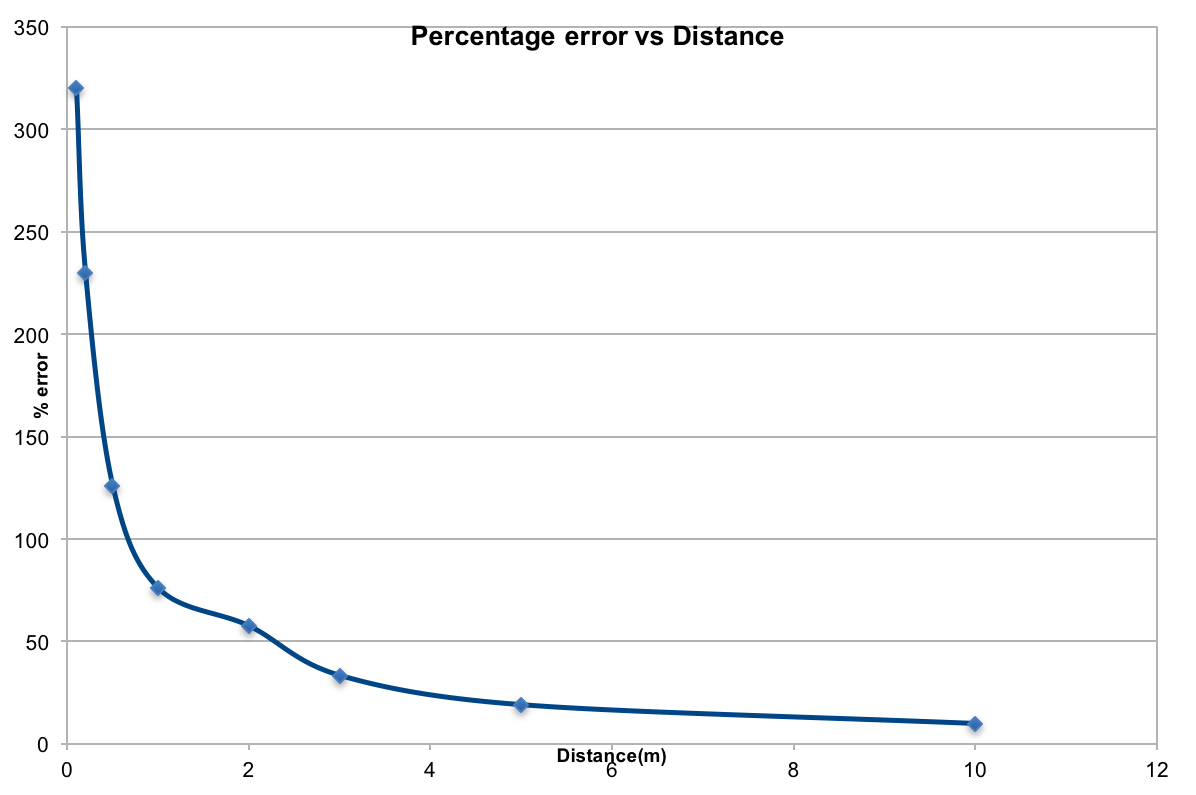
\includegraphics[width=3.5in]{errorcalibfig.png}
\caption{{Error Calibration for 2-way ranging}}
\label{errorcalib}
\end{figure}
We use this data to calibrate the ranges sent from mobile node to the admin laptop. The point-to-point distance between the tag node and each anchor node is calibrated using a look-up table. Error calibration using this technique increased the localization accuracy significantly. The error calibration increased the accuracy from 50 cm on all three axes to 20 cm on an average.




\subsection{Localization}

\begin{figure}[!h]
\centering
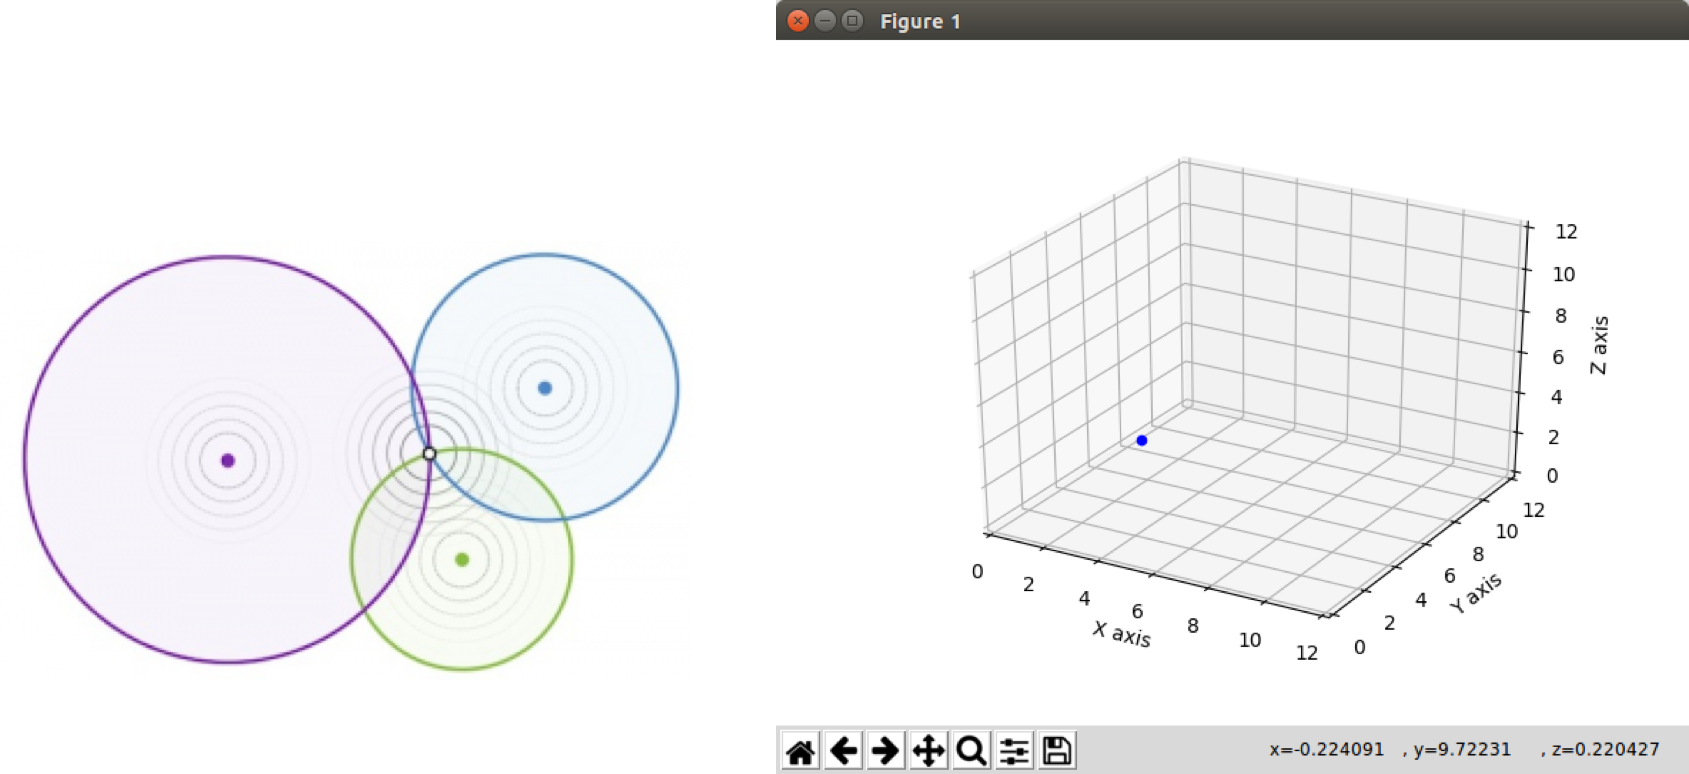
\includegraphics[width=3.5in]{3D_localization.png}
\caption{{3-D Localization}}
\label{3dlocalization}
\end{figure}


\subsection{Placement of Anchor Nodes}
\begin{figure}[!h]
\centering
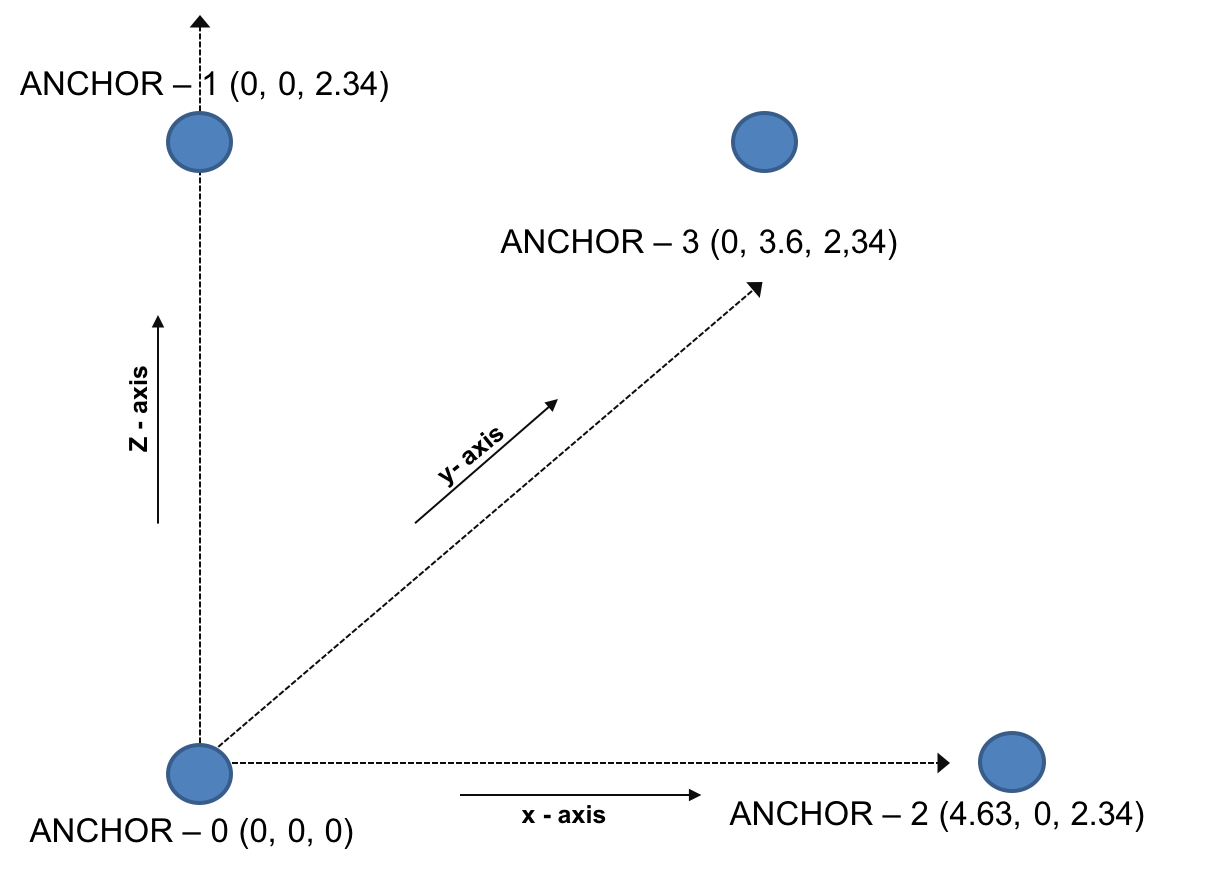
\includegraphics[width=3.5in]{anchorplacements.png}
\caption{{Placement of four Anchor Nodes}}
\label{anchorplacement}
\end{figure}


\section{Goals}
The Goals of the project are listed below: 

\begin{itemize}
    \item Goal : In our final project presentation, we plan to demonstrate the localization task performed by our system on a GUI. As the mobile node moves, the location of the node on the GUI will get updated in real-time.
    \item Stretch Goal 1 : Due to the inherent nature of the ToF algorithm, it will not be scalable when the number of mobile nodes are significantly high. With ToF, the anchor nodes have to send packets to all nodes with accurate time-stamps when the mobile nodes request for it. An efficient algorithm called Time Difference of Arrival(TDOA) can be used to overcome this problem. 
    \item Stretch Goal 2 : The crystals used on the DWM1000 for generating the clock frequency will have different performance on each board, which may result in inaccurate time-stamps. Due to this variance, the distance calculated may be quite inaccurate. If the error is too high, the localization will be way off. If this problem arises, we plan to synchronize the clocks across all DWM1000 modules externally to improve the accuracy.    
\end{itemize}
\section{Milestones}
The following are the milestones expected in course of the project:
\begin{itemize}
    \item Interface of DWM1000 with CC3200, \today : The DWM1000 modules have to be interfaced over the SPI interface with the CC3200 MCUs. This might require significant work in porting the SPI libraries from the reference STM32F105 board to TI CC3200 board.
    \item Distance measurement between two nodes (Mid-term Milestone) : The DWM1000 modules have to configured to work in the TOF mode. We plan to complete the distance measurement between two nodes with direct communication. In our demonstration during the mid-term project presentation, we plan to demonstrate the accuracy of distance measurement with the DWM1000 modules.
    \item Application Development for Localization (Final Project presentation) : Once the point-to-point communication is established and distance measurement between two nodes is done, we plan to build on this to implement our final application code. The final application code running on the mobile node will calculate the distance between itself and multiple anchor nodes. This data is sent to a PC to perform localization and compute the location of the mobile node. 

\end{itemize}
\section{Work Partitioning}
We plan to divide the work among the three team members as follows:
\begin{itemize}
    \item One team member will work on interfacing the CC3200 with the PC and get the GUI running. 
    \item Second team member will work on porting the code required for DWM1000 from reference solution to CC3200
    \item Third team member will work on hardware interfacing of DWM1000 with CC3200.
\end{itemize}




% An example of a floating figure using the graphicx package.
% Note that \label must occur AFTER (or within) \caption.
% For figures, \caption should occur after the \includegraphics.
% Note that IEEEtran v1.7 and later has special internal code that
% is designed to preserve the operation of \label within \caption
% even when the captionsoff option is in effect. However, because
% of issues like this, it may be the safest practice to put all your
% \label just after \caption rather than within \caption{}.
%
% Reminder: the "draftcls" or "draftclsnofoot", not "draft", class
% option should be used if it is desired that the figures are to be
% displayed while in draft mode.
%
%\begin{figure}[!t]
%\centering
%\includegraphics[width=2.5in]{myfigure}
% where an .eps filename suffix will be assumed under latex, 
% and a .pdf suffix will be assumed for pdflatex; or what has been declared
% via \DeclareGraphicsExtensions.
%\caption{Simulation results for the network.}
%\label{fig_sim}
%\end{figure}

% Note that the IEEE typically puts floats only at the top, even when this
% results in a large percentage of a column being occupied by floats.


% An example of a double column floating figure using two subfigures.
% (The subfig.sty package must be loaded for this to work.)
% The subfigure \label commands are set within each subfloat command,
% and the \label for the overall figure must come after \caption.
% \hfil is used as a separator to get equal spacing.
% Watch out that the combined width of all the subfigures on a 
% line do not exceed the text width or a line break will occur.
%
%\begin{figure*}[!t]
%\centering
%\subfloat[Case I]{\includegraphics[width=2.5in]{box}%
%\label{fig_first_case}}
%\hfil
%\subfloat[Case II]{\includegraphics[width=2.5in]{box}%
%\label{fig_second_case}}
%\caption{Simulation results for the network.}
%\label{fig_sim}
%\end{figure*}
%
% Note that often IEEE papers with subfigures do not employ subfigure
% captions (using the optional argument to \subfloat[]), but instead will
% reference/describe all of them (a), (b), etc., within the main caption.
% Be aware that for subfig.sty to generate the (a), (b), etc., subfigure
% labels, the optional argument to \subfloat must be present. If a
% subcaption is not desired, just leave its contents blank,
% e.g., \subfloat[].


% An example of a floating table. Note that, for IEEE style tables, the
% \caption command should come BEFORE the table and, given that table
% captions serve much like titles, are usually capitalized except for words
% such as a, an, and, as, at, but, by, for, in, nor, of, on, or, the, to
% and up, which are usually not capitalized unless they are the first or
% last word of the caption. Table text will default to \footnotesize as
% the IEEE normally uses this smaller font for tables.
% The \label must come after \caption as always.
%
%\begin{table}[!t]
%% increase table row spacing, adjust to taste
%\renewcommand{\arraystretch}{1.3}
% if using array.sty, it might be a good idea to tweak the value of
% \extrarowheight as needed to properly center the text within the cells
%\caption{An Example of a Table}
%\label{table_example}
%\centering
%% Some packages, such as MDW tools, offer better commands for making tables
%% than the plain LaTeX2e tabular which is used here.
%\begin{tabular}{|c||c|}
%\hline
%One & Two\\
%\hline
%Three & Four\\
%\hline
%\end{tabular}
%\end{table}


% Note that the IEEE does not put floats in the very first column
% - or typically anywhere on the first page for that matter. Also,
% in-text middle ("here") positioning is typically not used, but it
% is allowed and encouraged for Computer Society conferences (but
% not Computer Society journals). Most IEEE journals/conferences use
% top floats exclusively. 
% Note that, LaTeX2e, unlike IEEE journals/conferences, places
% footnotes above bottom floats. This can be corrected via the
% \fnbelowfloat command of the stfloats package.



% if have a single appendix:
%\appendix[Proof of the Zonklar Equations]
% or
%\appendix  % for no appendix heading
% do not use \section anymore after \appendix, only \section*
% is possibly needed

% use appendices with more than one appendix
% then use \section to start each appendix
% you must declare a \section before using any
% \subsection or using \label (\appendices by itself
% starts a section numbered zero.)
%





% trigger a \newpage just before the given reference
% number - used to balance the columns on the last page
% adjust value as needed - may need to be readjusted if
% the document is modified later
%\IEEEtriggeratref{8}
% The "triggered" command can be changed if desired:
%\IEEEtriggercmd{\enlargethispage{-5in}}

% references section

% can use a bibliography generated by BibTeX as a .bbl file
% BibTeX documentation can be easily obtained at:
% http://mirror.ctan.org/biblio/bibtex/contrib/doc/
% The IEEEtran BibTeX style support page is at:
% http://www.michaelshell.org/tex/ieeetran/bibtex/
\bibliographystyle{IEEEtran}
% argument is your BibTeX string definitions and bibliography database(s)
%\printbibliography
\bibliography{refer}
%
% <OR> manually copy in the resultant .bbl file
% set second argument of \begin to the number of references
% (used to reserve space for the reference number labels box)
% \begin{thebibliography}{1}

% \bibitem{IEEEhowto:kopka}
% H.~Kopka and P.~W. Daly, \emph{A Guide to \LaTeX}, 3rd~ed.\hskip 1em plus
%   0.5em minus 0.4em\relax Harlow, England: Addison-Wesley, 1999.

% \end{thebibliography}
%\bibliographystyle{unsrt}

%\begin{thebibliography}{1}
%
%  \bibitem{IEEE} Lazik, Patrick and Rajagopal, Niranjini and Shih, Oliver and Sinopoli, Bruno and Rowe, Anthony \emph{ALPS: A bluetooth and ultrasound platform for mapping and localization}, \hskip Proceedings of the 13th ACM Conference on Embedded Networked Sensor Systems
%  \bibitem{IEEE2} Rajagopal, Niranjini and Chayapathy, Sindhura and Sinopoli, Bruno and Rowe, Anthony \emph{Beacon placement for range-based indoor localization}, \hskip ndoor Positioning and Indoor Navigation (IPIN), 2016 International Conference
%  \bibitem{IEEE3} Lazik, Patrick and Rajagopal, Niranjini and Sinopoli, Bruno and Rowe, Anthony \emph{Ultrasonic time synchronization and ranging on smartphones}, \hskip Real-Time and Embedded Technology and Applications Symposium (RTAS), 2015 IEEE
%  \bibitem{IEEE4} Ye, Tingcong and Walsh, Michael and Haigh, Peter and Barton, John and O'Flynn, Brendan \emph{Experimental impulse radio IEEE 802.15. 4a UWB based wireless sensor localization technology: Characterization, reliability and ranging}, \hskip ISSC 2011, 22nd IET Irish Signals and Systems Conference, Dublin, Ireland. 23-24 Jun 2011
%\end{thebibliography}



% biography section
% 
% If you have an EPS/PDF photo (graphicx package needed) extra braces are
% needed around the contents of the optional argument to biography to prevent
% the LaTeX parser from getting confused when it sees the complicated
% \includegraphics command within an optional argument. (You could create
% your own custom macro containing the \includegraphics command to make things
% simpler here.)
%\begin{IEEEbiography}[{\includegraphics[width=1in,height=1.25in,clip,keepaspectratio]{mshell}}]{Michael Shell}
% or if you just want to reserve a space for a photo:


% You can push biographies down or up by placing
% a \vfill before or after them. The appropriate
% use of \vfill depends on what kind of text is
% on the last page and whether or not the columns
% are being equalized.

%\vfill

% Can be used to pull up biographies so that the bottom of the last one
% is flush with the other column.
%\enlargethispage{-5in}



% that's all folks
\end{document}